\section{SEIR modelling with mixing matrices}

Starting from the 1-community SEIR model, the following diff equations can be set up:

\begin{align*}
\dv{t}S(t) =& - 1/N \beta I(t) S(t) \\
\dv{t}E(t) =& 1/N \beta I(t)S(t) - \eta a E(t) \\
\dv{t}I(t) =& \eta a E(t) - \gamma I(t) \\
\dv{t}R(t) =& \gamma I(t)
\end{align*}

where $a$ is reciprocal incubation time,
$\beta$ is reciprocal time between contact,
$\gamma$ is reciprocal recovery time,
and $\eta$ is efficiancy of infection (the proportion of exposed population becoming vectors of the diease).
Note that we here assume a consant population:

\begin{align*}
S(t) + E(t) + I(t) + R(t) = N \quad , \quad \forall t \in \left[ 0, \infty \right[ %\\
% \dv{t} \left( S(t) + E(t) + I(t) + R(t) \right) = 0
\end{align*}

This model is for one homogenous population, and so to refine it, we now consider a modified model in which wh have several different communities\footnote{the communities we consider here are different age groups.}, all with their separate evolution system, such that the population in each community, is constant:

\begin{align*}
\dv{t}S_{i}(t) =& - 1/N_{i} \beta I^{M}_{i}(t) S_{i}(t) \\
\dv{t}E_{i}(t) =& 1/N_{i} \beta I^{M}_{i}(t)S_{i}(t) - \eta a E_{i}(t) \\
\dv{t}I_{i}(t) =& \eta a E_{i}(t) - \gamma I_{i}(t) \\
\dv{t}R_{i}(t) =& \gamma I_{i}(t)
\end{align*}

where in this model, the rate of exposiure is determined by the new quantity $I_{T}(t)$ that constitute the wheigted proprtion of the infectious population, given as:

\begin{align*}
I^{M}_{j}(t) = \sum_{f}\sum_{i}w^{f}_{j}(c^{f}_{ij})^{T}I_{i}(t)
\end{align*}

where the indices $i,j$ indicates the different age groups, and the index $f$, indicates the \textit{form of transmition}\footnote{or rather the context/sitution/type/incident. pick the one you like best.}, which can be picked as combinations from the folowing table:

\begin{table}[H]
\centering
\begin{tabular}{l | *{4}{c}}
\hline \\
Infection wheights & school (s) & work (w) & home (h) & other (o) \\
\hline \\
Physical (p) ($\times 1$)& 1 & 0.5 & 1 & 0.2 \\
Casual (c) ($\times 0.2$) & 0.2 & 0.1 & 0.2 & 0.04
\end{tabular}
\end{table}
This can now be vectorized as follows:

\begin{align*}
w_{i} = (w_{ps}, w_{pw}, w_{ph}, w_{po}, w_{cs}, w_{cw}, w_{ch}, w_{co})^{T}
\end{align*}

where the subscript indicates the product between the corresponding partial whaights, e.g. $w_{ph} = w_{p} w_{h}$.
The index indicating the different age groups is necessary if different stategies are emplored by different age groups e.g. the age group 0-9 yrs are allowed in school, while age group 10-19 yrs are not, which corresponds to setting the coorsponding school-wheights to zero for the latter group, but not the first.

With this in place, a script is made and the age-differentiated SEIR-model is is integrated numerically, using scipy-odeint package, with the following results:

\newpage

The weights described above, used in the scenario is:
\begin{table}[H]
\centering
\input{../meta/w_table_n.txt}
\end{table}

\begin{figure}[H]
\centering
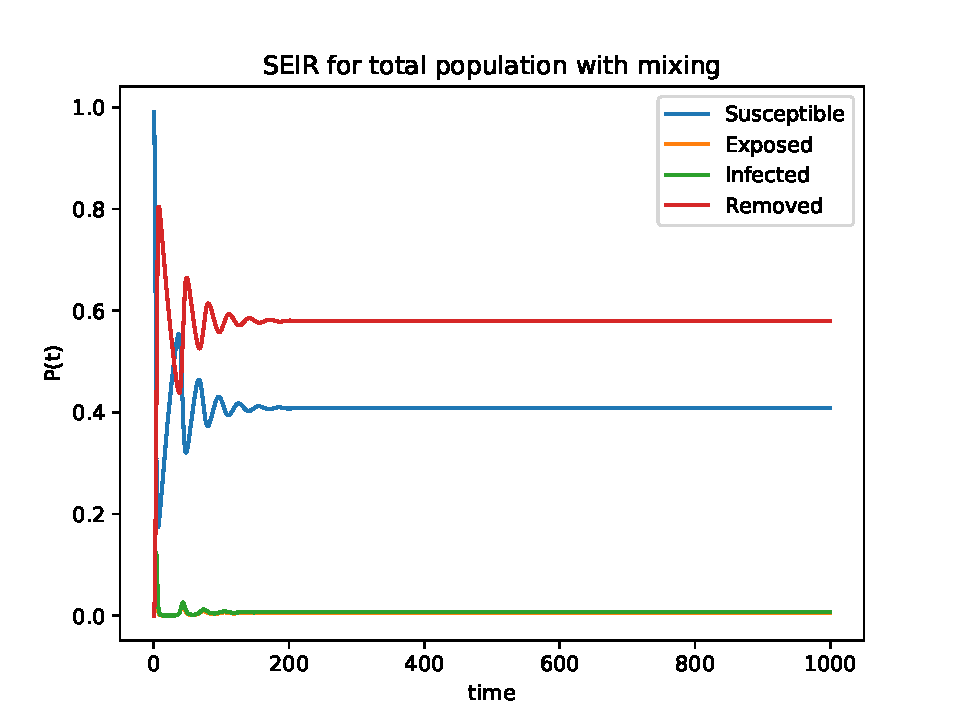
\includegraphics[width = 0.75\textwidth]{../fig/SEIR_total_population_mix_n.pdf}
\caption{
\protect\input{../fig/SEIR_total_population_mix_figtext_n.txt} 
\label{fig:total_pop_mix_n}}
\end{figure}

\begin{figure}[H]
\centering
\begin{subfigure}{0.40\textwidth}
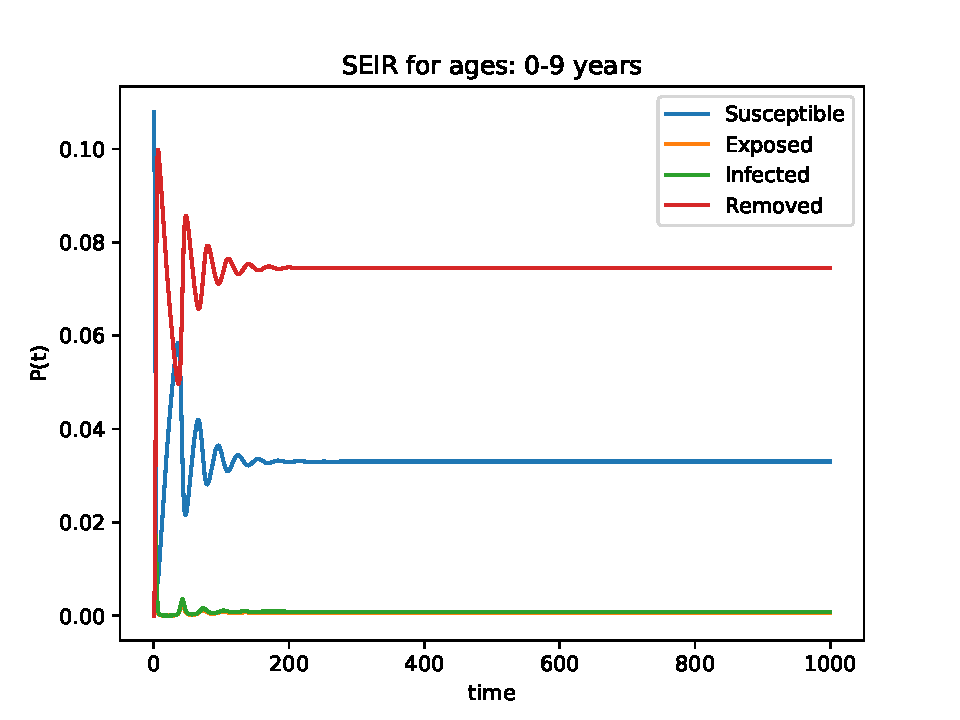
\includegraphics[width = \textwidth]{../fig/SEIR_0-9_n.pdf}
\caption{\protect\input{../fig/SEIR_0-9_figtext_n.txt}}
\end{subfigure}
\begin{subfigure}{0.40\textwidth}
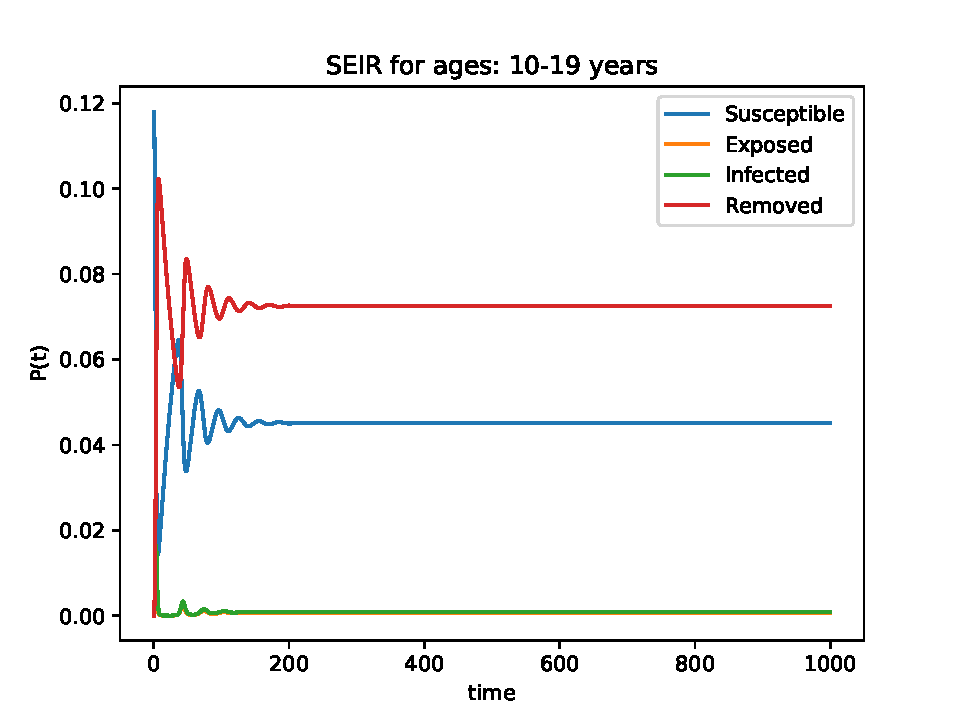
\includegraphics[width = \textwidth]{../fig/SEIR_10-19_n.pdf}
\caption{\protect\input{../fig/SEIR_10-19_figtext_n.txt}}
\end{subfigure}
\begin{subfigure}{0.40\textwidth}
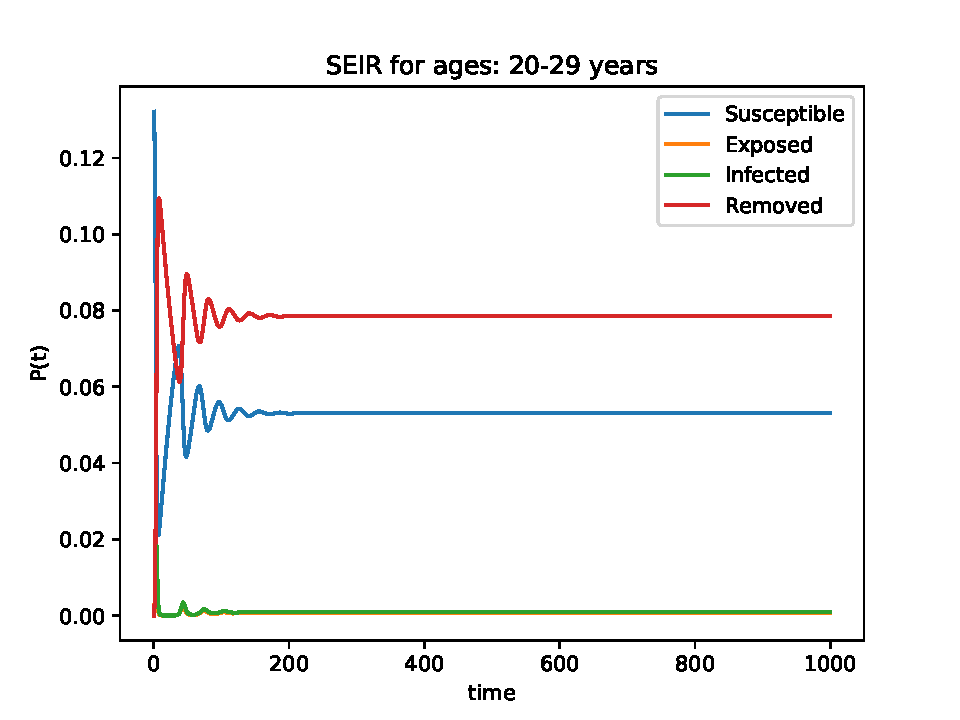
\includegraphics[width = \textwidth]{../fig/SEIR_20-29_n.pdf}
\caption{\protect\input{../fig/SEIR_20-29_figtext_n.txt}}
\end{subfigure}
\begin{subfigure}{0.40\textwidth}
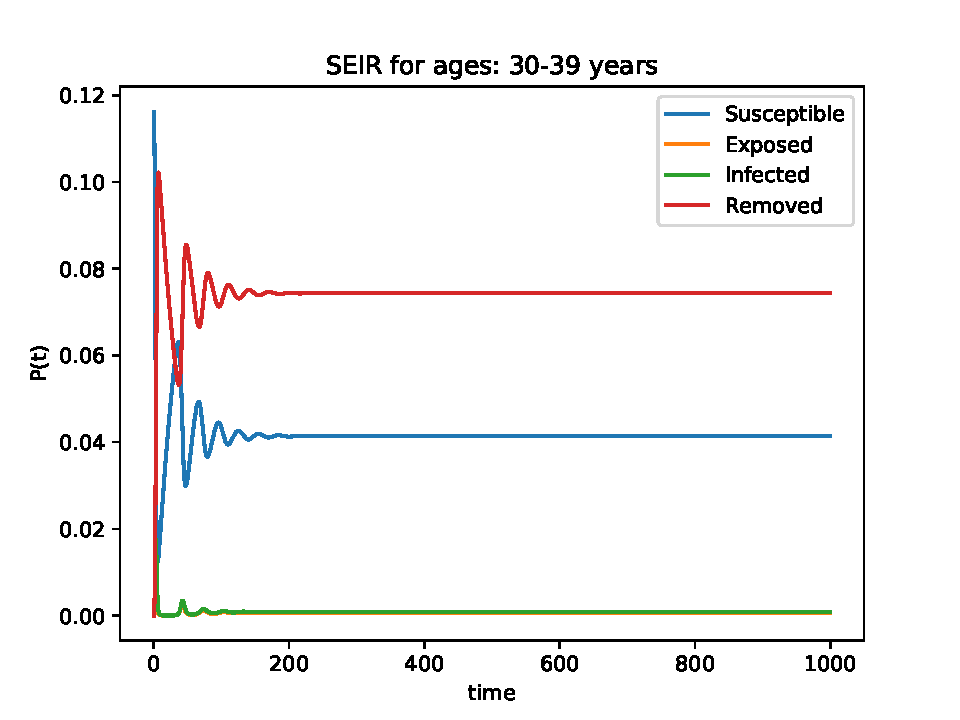
\includegraphics[width = \textwidth]{../fig/SEIR_30-39_n.pdf}
\caption{\protect\input{../fig/SEIR_30-39_figtext_n.txt}}
\end{subfigure}
\begin{subfigure}{0.40\textwidth}
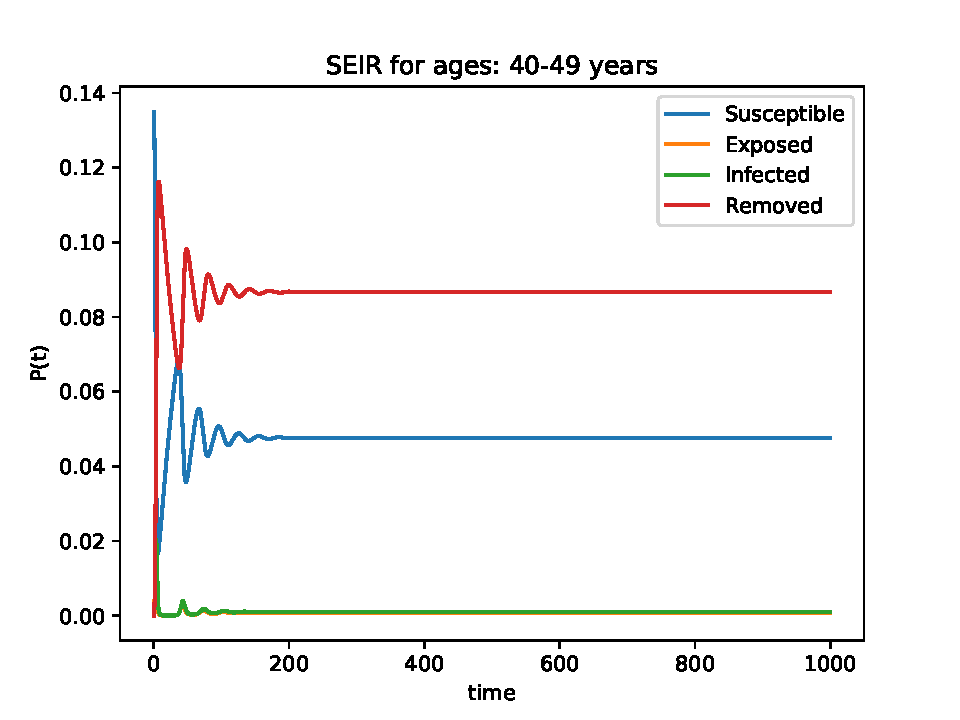
\includegraphics[width = \textwidth]{../fig/SEIR_40-49_n.pdf}
\caption{\protect\input{../fig/SEIR_40-49_figtext_n.txt}}
\end{subfigure}
\begin{subfigure}{0.40\textwidth}
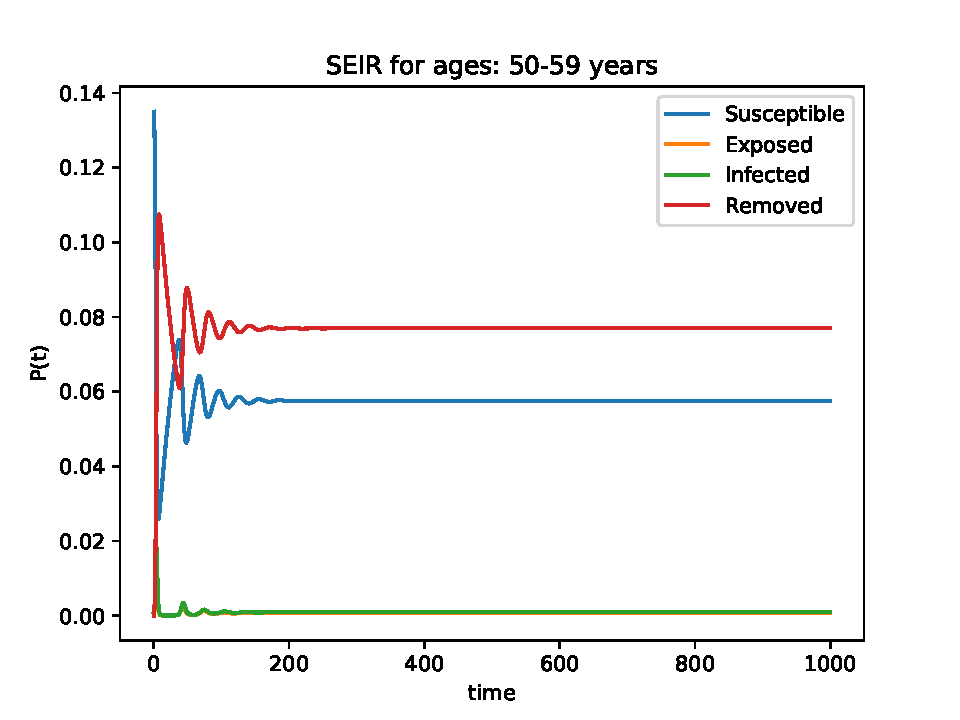
\includegraphics[width = \textwidth]{../fig/SEIR_50-59_n.pdf}
\caption{\protect\input{../fig/SEIR_50-59_figtext_n.txt}}
\end{subfigure}
\begin{subfigure}{0.40\textwidth}
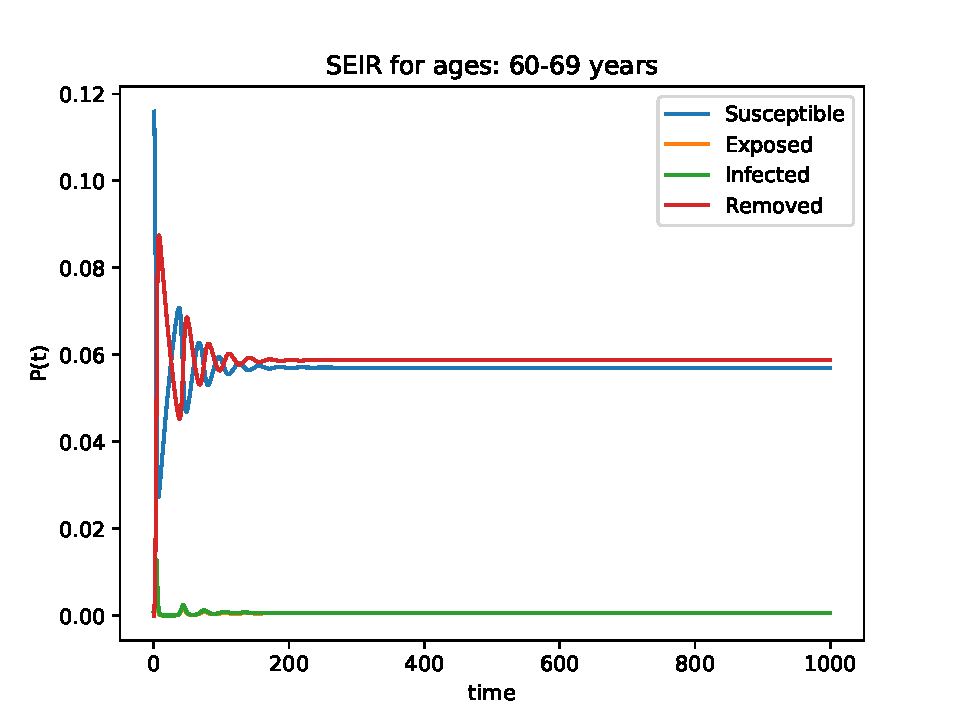
\includegraphics[width = \textwidth]{../fig/SEIR_60-69_n.pdf}
\caption{\protect\input{../fig/SEIR_60-69_figtext_n.txt}}
\end{subfigure}
\begin{subfigure}{0.40\textwidth}
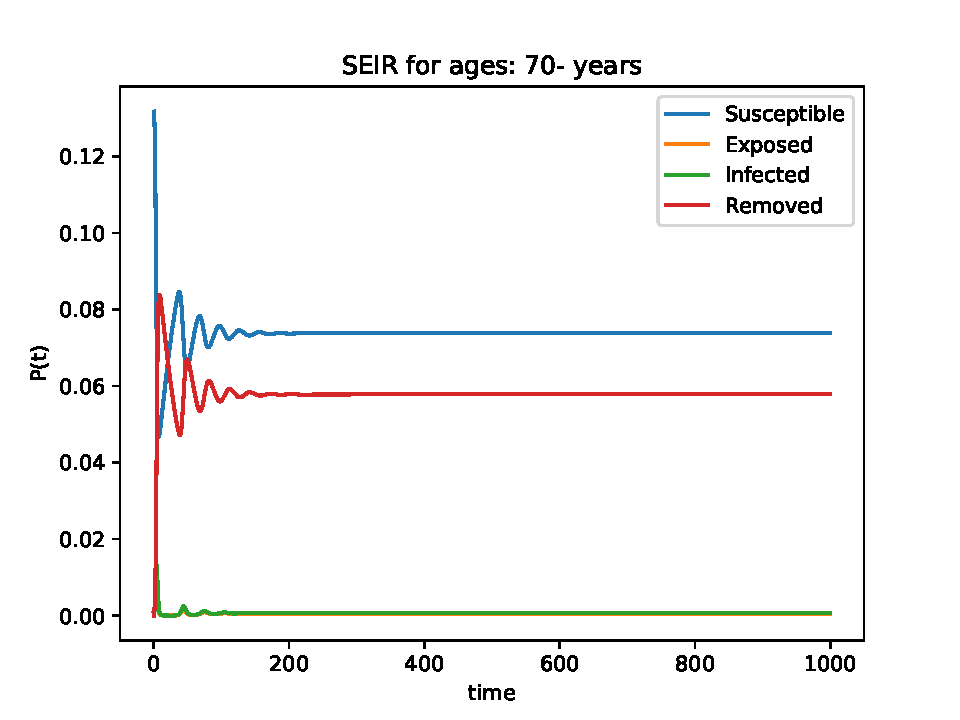
\includegraphics[width = \textwidth]{../fig/SEIR_70-_n.pdf}
\caption{\protect\input{../fig/SEIR_70-_figtext_n.txt}}
\end{subfigure}
\end{figure}

% --

\newpage

The weights described above, used in the scenario is:
\begin{table}[H]
\centering
\input{../meta/w_table_q.txt}
\end{table}

\begin{figure}[H]
\centering
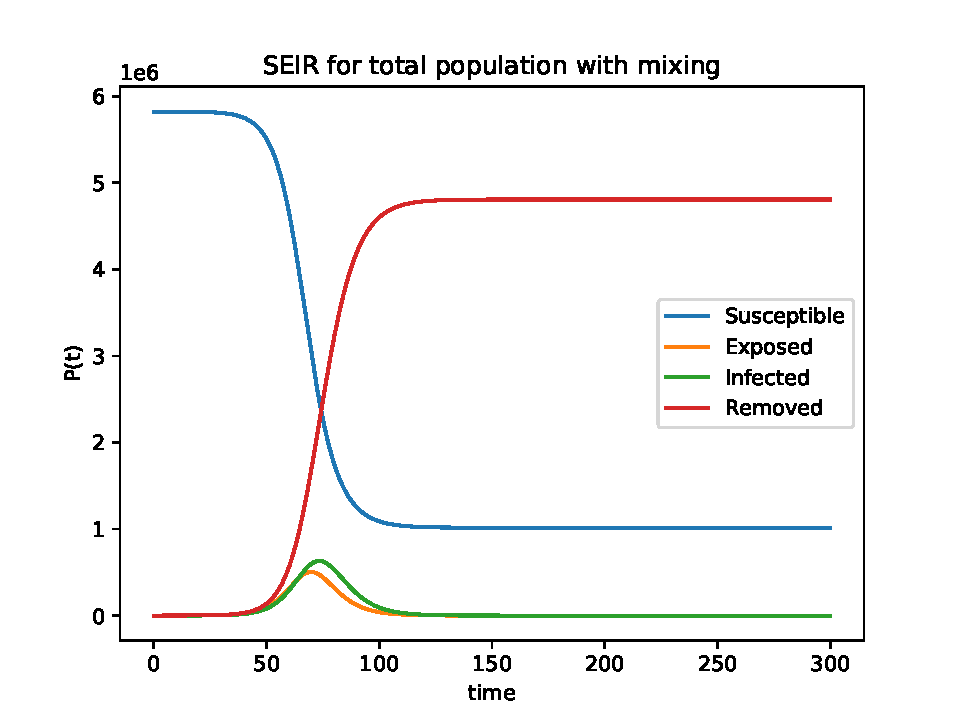
\includegraphics[width = 0.75\textwidth]{../fig/SEIR_total_population_mix_q.pdf}
\caption{
\protect\input{../fig/SEIR_total_population_mix_figtext_q.txt} 
\label{fig:total_pop_mix_q}}
\end{figure}

\begin{figure}[H]
\centering
\begin{subfigure}{0.40\textwidth}
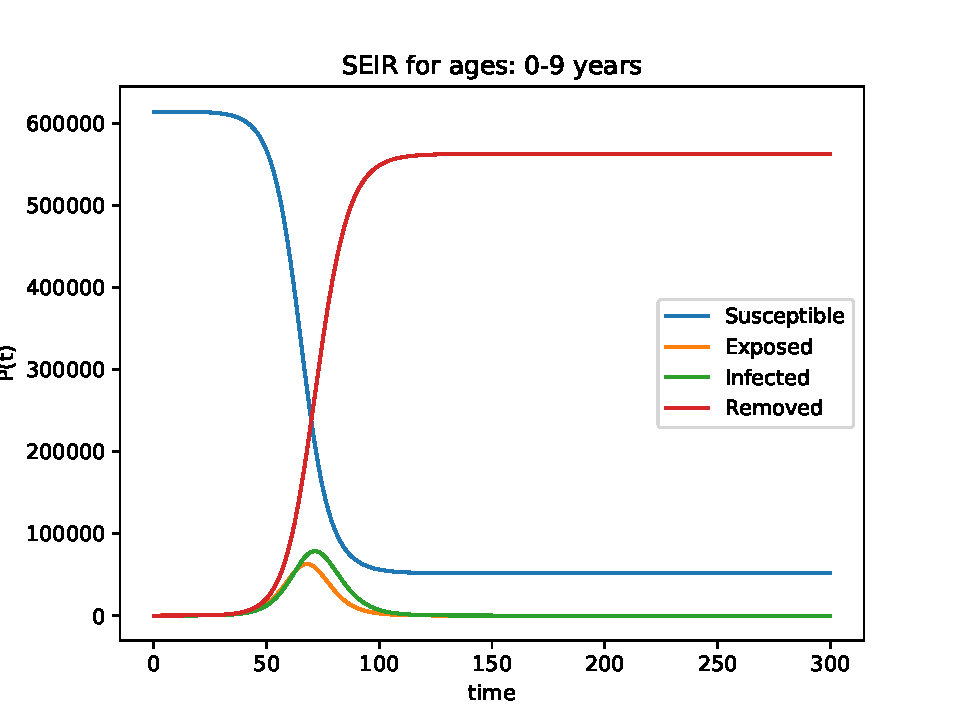
\includegraphics[width = \textwidth]{../fig/SEIR_0-9_q.pdf}
\caption{\protect\input{../fig/SEIR_0-9_figtext_q.txt}}
\end{subfigure}
\begin{subfigure}{0.40\textwidth}
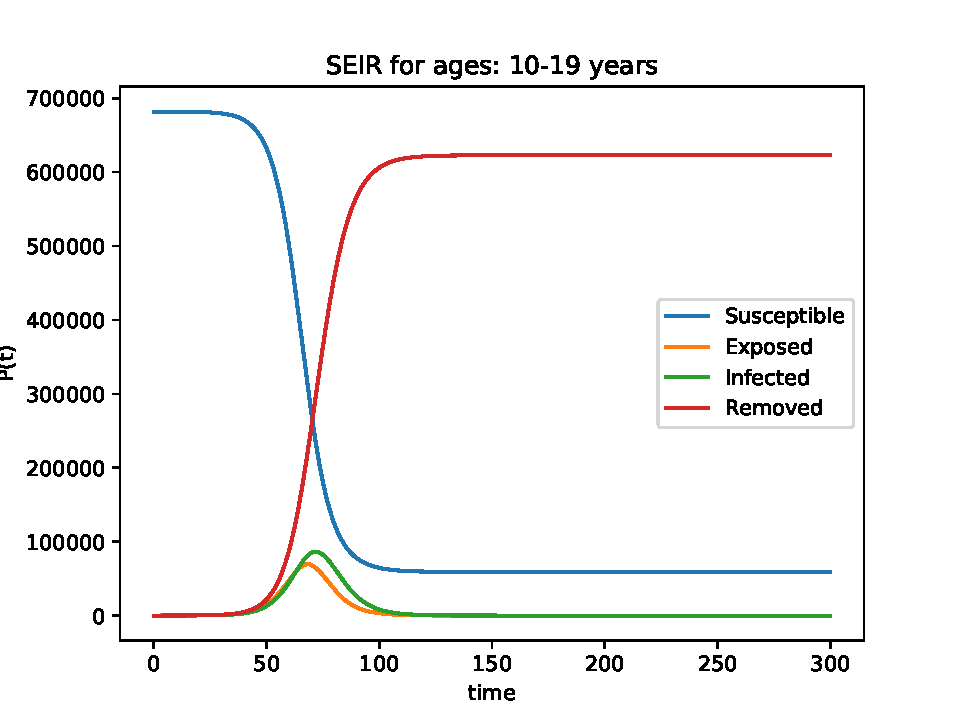
\includegraphics[width = \textwidth]{../fig/SEIR_10-19_q.pdf}
\caption{\protect\input{../fig/SEIR_10-19_figtext_q.txt}}
\end{subfigure}
\begin{subfigure}{0.40\textwidth}
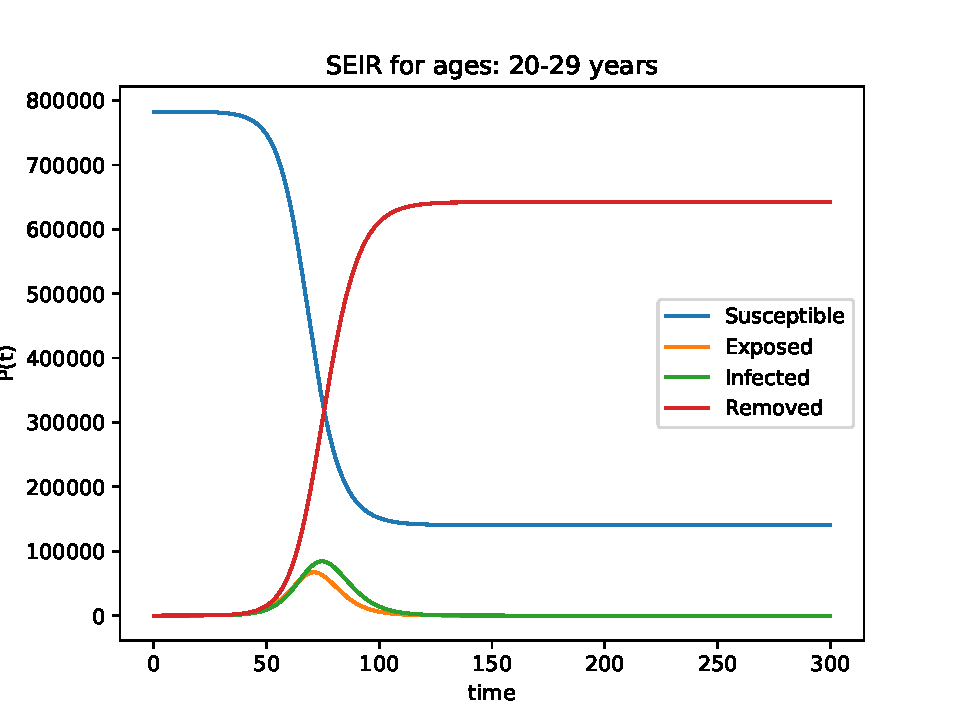
\includegraphics[width = \textwidth]{../fig/SEIR_20-29_q.pdf}
\caption{\protect\input{../fig/SEIR_20-29_figtext_q.txt}}
\end{subfigure}
\begin{subfigure}{0.40\textwidth}
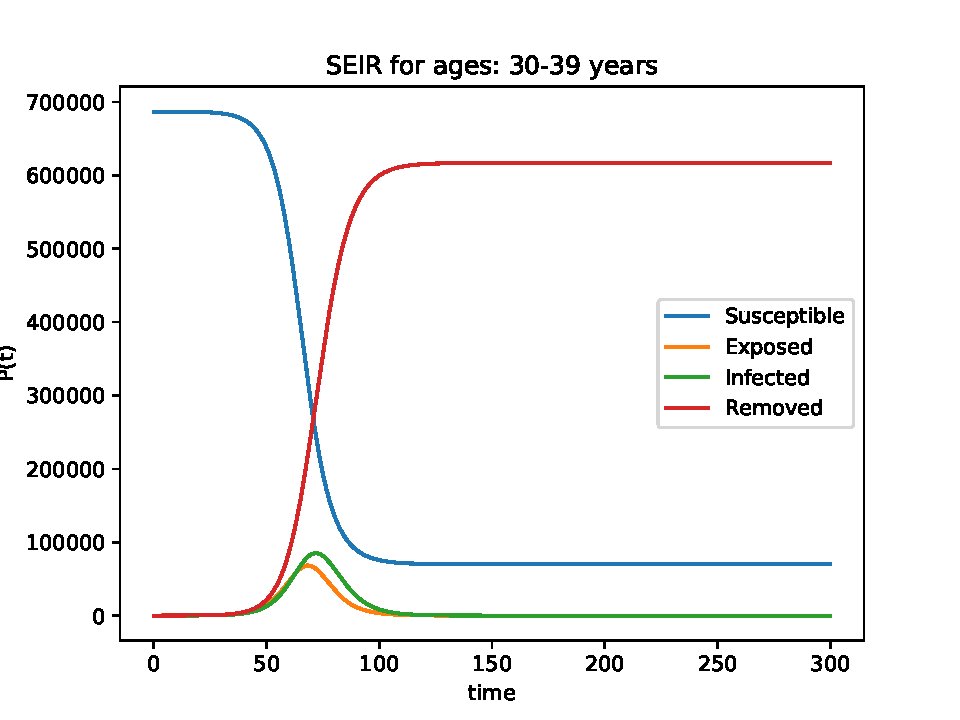
\includegraphics[width = \textwidth]{../fig/SEIR_30-39_q.pdf}
\caption{\protect\input{../fig/SEIR_30-39_figtext_q.txt}}
\end{subfigure}
\begin{subfigure}{0.40\textwidth}
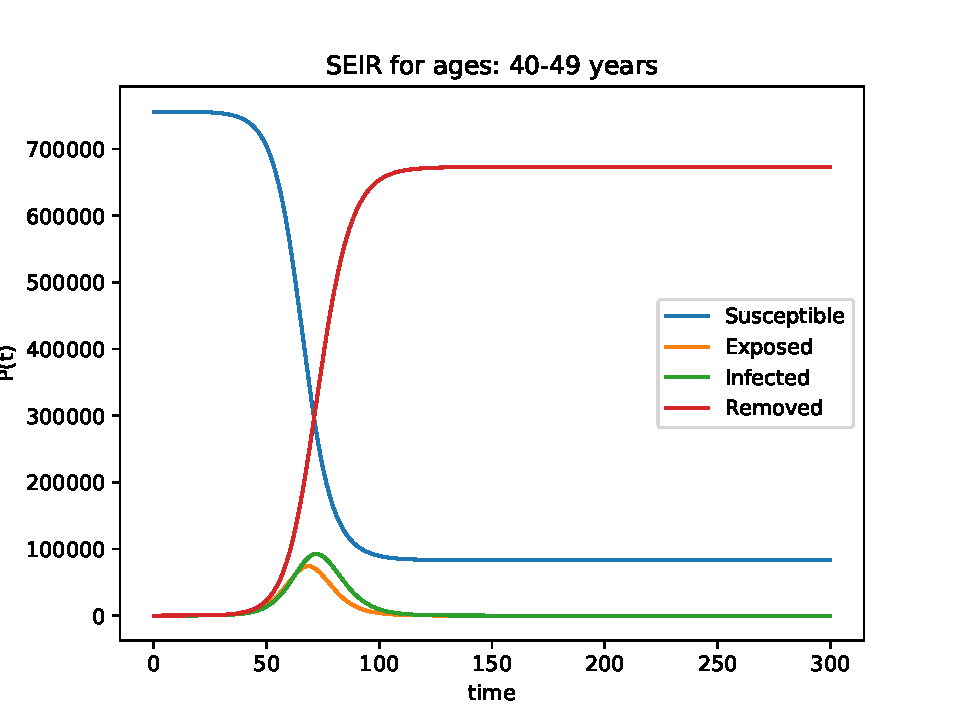
\includegraphics[width = \textwidth]{../fig/SEIR_40-49_q.pdf}
\caption{\protect\input{../fig/SEIR_40-49_figtext_q.txt}}
\end{subfigure}
\begin{subfigure}{0.40\textwidth}
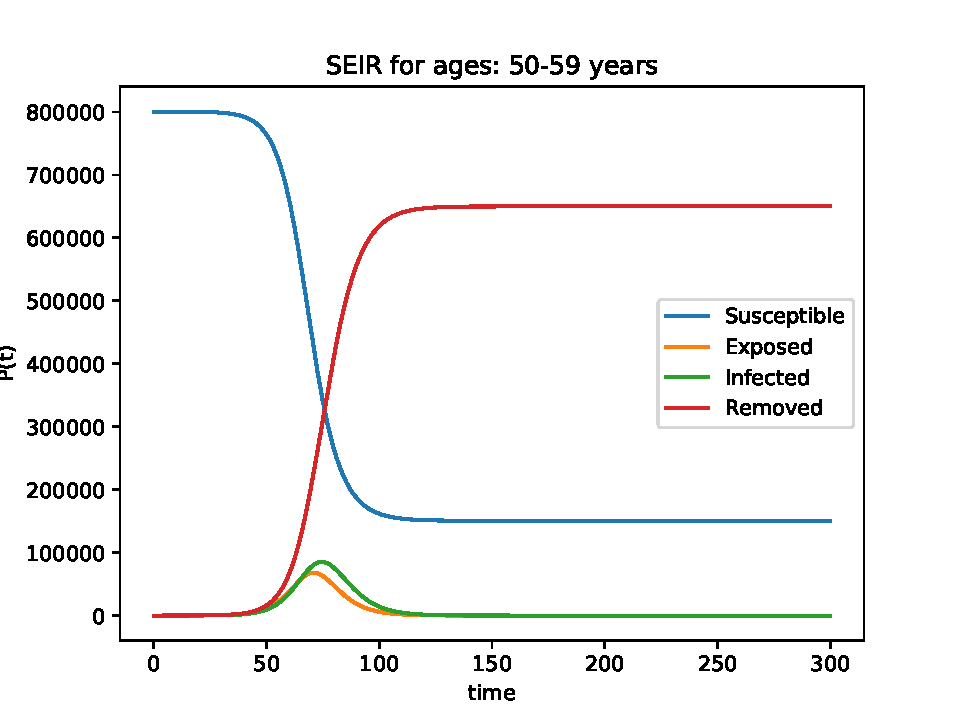
\includegraphics[width = \textwidth]{../fig/SEIR_50-59_q.pdf}
\caption{\protect\input{../fig/SEIR_50-59_figtext_q.txt}}
\end{subfigure}
\begin{subfigure}{0.40\textwidth}
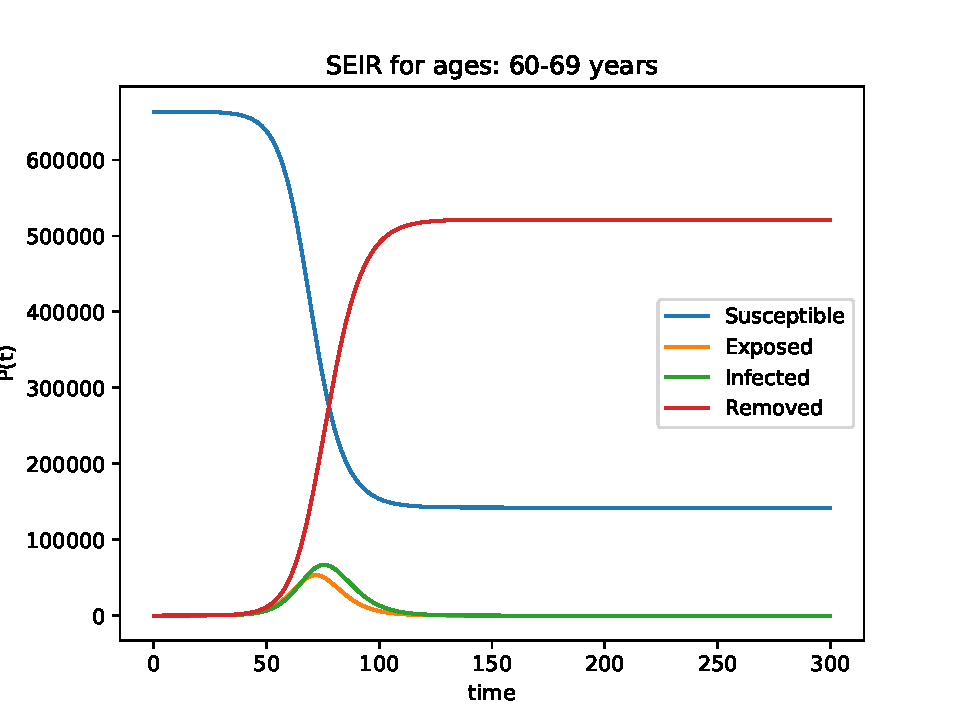
\includegraphics[width = \textwidth]{../fig/SEIR_60-69_q.pdf}
\caption{\protect\input{../fig/SEIR_60-69_figtext_q.txt}}
\end{subfigure}
\begin{subfigure}{0.40\textwidth}
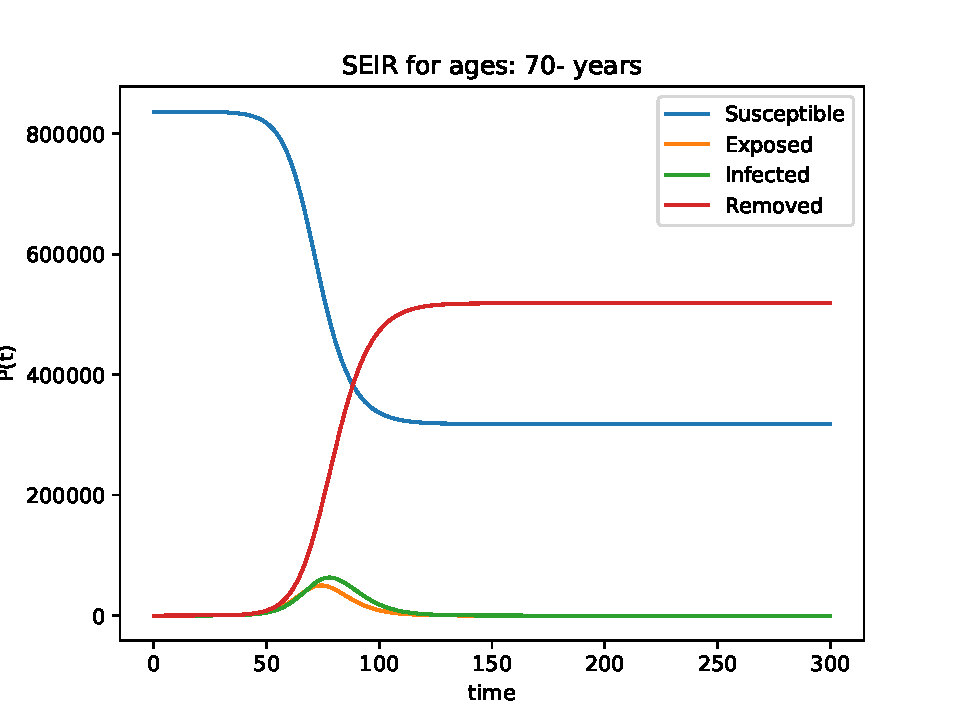
\includegraphics[width = \textwidth]{../fig/SEIR_70-_q.pdf}
\caption{\protect\input{../fig/SEIR_70-_figtext_q.txt}}
\end{subfigure}
\end{figure}
